\addchapheadtotoc
\chapter{Introduction}
\section{Context}
An operating system (\acrshort {os}) is a set of computer programs that contribute to optimal use of the machine by user's applications. In general, it is the master of the system and as this, it can do privileged actions that other generic softwares cannot. Examples of operating systems: Ubuntu, Windows, Android, etc. Examples of privileged actions that can only be done by the OS: shutting down the computer, shutting down the processor, allocating memory to an application, modifying the system date, communicating with external devices (copying a file from or to a USB memory stick), changing running program, etc.

An operating system is made up of a kernel which runs in privileged mode, and often but not always, of a set of pilot processes which allow to use the peripherals and of a set of service processes which serve as interfaces between applications on one hand, and the kernel and peripherals on the other hand. Privileged actions are defined by the CPU architecture. Executing in privileged mode means that when the processor is operating in this mode, the program can execute the privileged actions which we mentioned above.

Transient faults are change of state that affect the contents of a memory area or a control circuit in a micro-electronic device, such as in a microprocessor, semiconductor memory, or power transistors without damaging the component. As a result, the system remains in working state but includes erroneous data. Examples: one or more bits that change value in a memory area or a flip-flop that triggers sporadically a command. Transient faults results from an accumulation of electrical charges inside transistors that make electronic components. The accumulation can be caused by a flow of cosmic particles ejected by a sudden intensification of solar activity. This phenomenon is temporary and one could rewrite later in this affected memory area without any problem and the machine could also continue to function normally thereafter.

In environment irradiated by cosmic rays like space, transient faults are frequent so that no electronic component could function normally without undergoing transient faults unless it is equipped with special protections. They are generally used in planes, satellites and space probes. That is why electronic devices used in space programs are different from those we found in our common working place. Transient faults are less frequent at ground level, but some faults have already been reported as a result of their actions. The diminishing size and voltages in use in microchips increases their sensitivity to these phenomenons because the charge holding a bit of information becomes smaller and can more easily be changed by the charge transferred by a high energy particle colliding with the chip [Hei11] [VFR07]. 

Electronic components are therefore subject to transient faults, and these transient faults can induce errors in the execution of the programs running in these components, it is therefore necessary to protect either the components or the programs, but generally both, to ensure proper functioning of the system. We then talk about hardening the system.

Because of the high risk of transient faults in critical environments such as space, aeronautics or armaments, the computer components used in these fields are generally heavier, slower and more expensive than those found on the common market because they are produced in very small quantities for a niche market.

Successfully using ordinary equipment in these critical environments would therefore represent a significant financial gain. For example, the RAD750 on-board computer (figure \ref{fig:rad750}) of the "Curiosity Rover" probe (figure \ref{fig:curiosity_rover}) has a frequency of 200 MHz and costs \$US 200000 \cite{john_rhea} while an inexpensive Xeon type processor is multicore, can be clocked up to 4 GHz, and is sold at \$US 200.

\begin{minipage}[t]{0.48\textwidth} \begin{flushleft}\vspace{-2ex}
		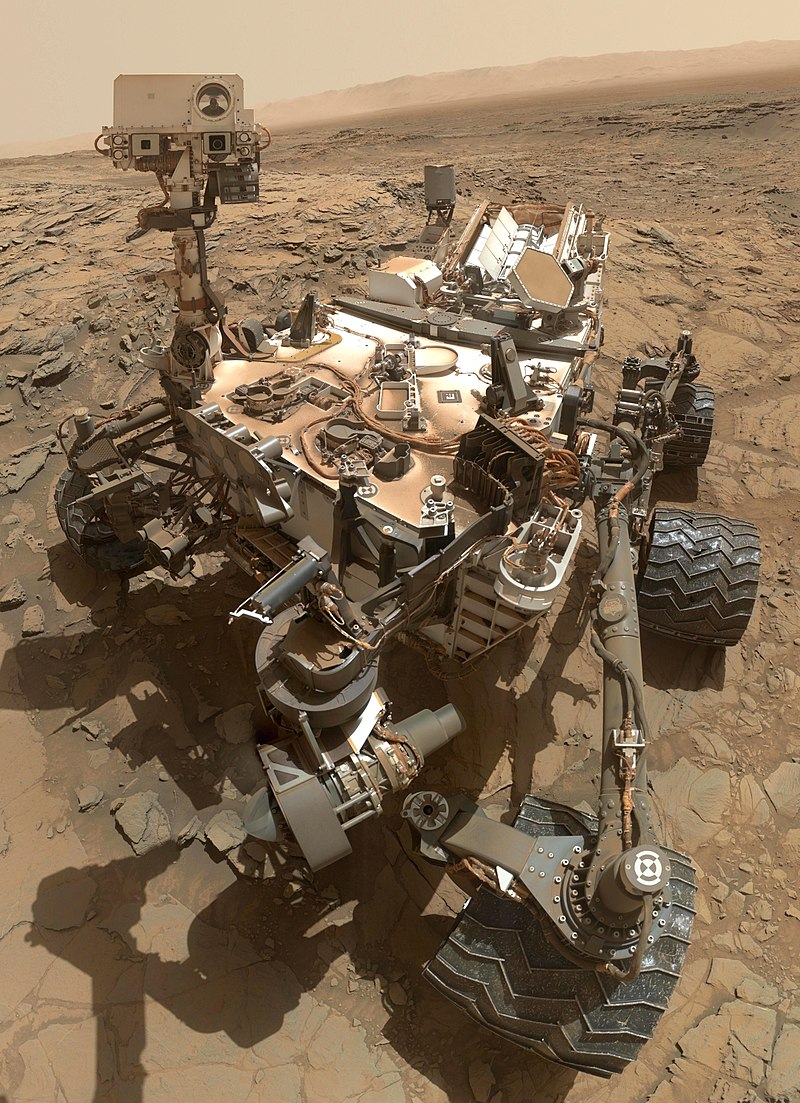
\includegraphics[width=0.8\textwidth]{image/curiosity_rover}
		\captionof{figure}{\\Self-portrait of Curiosity located at \\the foothill of Mount Sharp (October 6, 2015)}
		\label{fig:curiosity_rover}
\end{flushleft}\end{minipage}
\begin{minipage}[t]{0.48\textwidth} \begin{flushright}\vspace{-3ex}
		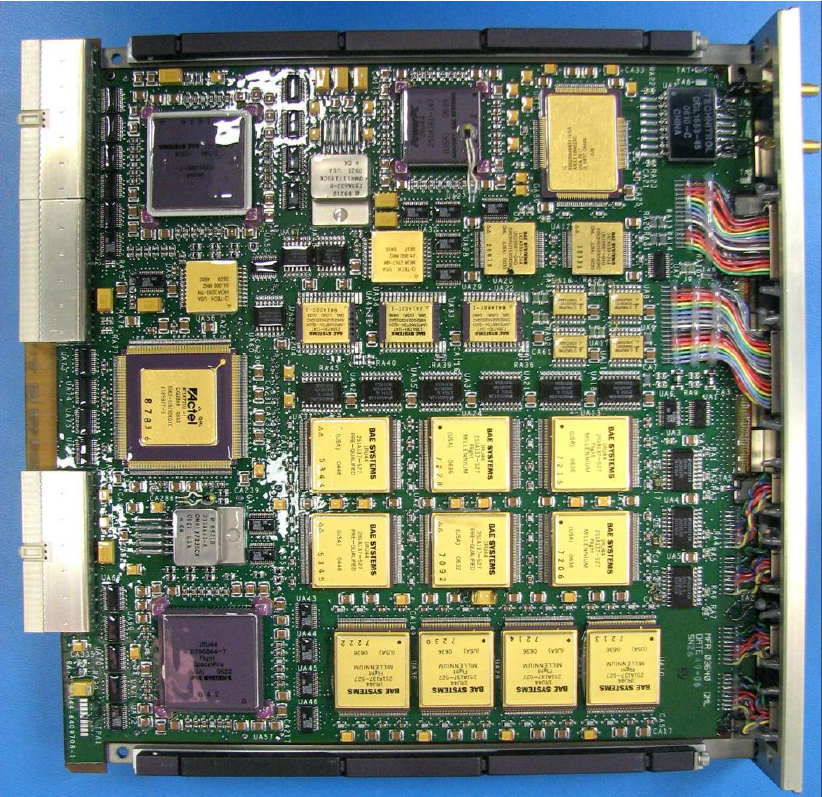
\includegraphics[width=1.1\textwidth]{image/RAD750}
		\vspace{0.05ex}
		\captionof{figure}{\\RAD750 onboard computer}
		\label{fig:rad750}
\end{flushright}\end{minipage}

Many researches has been carried out and has proposed solutions which essentially aim at making the program in execution insensitive to transient faults. We can cite for example the work of L. Lesage which resulted in a system for protecting a program which is executed directly on a bare machine. B. Döbel also proposed a solution of partial protection for applications in multitasking. E. Assogba has extended Döbel's solution to provide full protection for applications. However, all these works does not yet allow a total adoption of these protection methods because they do not address protecting the operating system itself which is essential in every current computing system. The present research therefore proposes to explore how to protect the OS and to offer a demonstration, and using the method of protection from recent work in the field, to also protect applications; all resulting in a fully protected computer system.

\section{Problematic}

There exist several techniques to guard against these kinds of error (to prevent them from occurring) or to mitigate their effects and a lot of research are being conducted in this field. But making a system totally resilient against all SEUs at minimum cost (on common-market devices), thus relying on software design, is still a challenge. Software based techniques are greatly appealing because they are cheaper than hardware ones \citep{Madeira2002ExperimentalEO}. They require no or little modification to the existing hardware and can be instantiated multiple times without expensive hardware manufacturing for special markets. Lesage et al. proposed in \citep{lesage_software_2011} a software based technique where a stand-alone program was made self-protected by resorting to double execution with comparison to detect and correct SEU errors. A thesis has being conducted to extend this technique to harden user application programs in a multi-task environment relying on common hardware features available in \acrfull{cots} processors \citep{emery_assogba}. 

Emery Assogba's research was based on the Minix micro-kernel operating system, which means that it is not reusable as it is. Likewise, those from Björn Döbel are based on the FIASCO.OC micro-kernel OS and are also therefore not reusable on other platforms \citep{dobel_can_2014}. Only applications running on these platforms can benefit from protection against transient faults.
On another level, by analyzing the used techniques, we realize that they cannot be used to protect an operating system since they rather use the functionality of OS in other to protect applicztions.
It is for these reasons that this thesis was started to answer the fundamental question of how to protect an operating system, and by this way, also the applications running on it.

Our main goal in this research is to explore how we can protect an entire unmodified \acrfull{os} at run-time against SEU by resorting to mainly software based techniques combined with some simple available features on the hardware. This is the principle of the blended hardening technique. Assuming a properly hardened memory, the blended hardening technique is based on dividing each running process in short processing elements, short enough to be, with a very high probability, only subject to, at most, a single SEU. To achieve this, we rely on a systematic redundancy technique called \acrfull{dwc} of relatively short sequences of instructions called \acrfull{pe}, to detect and recover from any occurring error. Unlike other redundancy schemes, this technique aims to introduce systematic redundancy at a rather thin time granularity (in terms of hundreds of \SI{}{\micro\second}) while satisfying real time constraint required by user applications. The two runs of a PE plus their comparison forms an \acrfull{ot} that should be kept atomic.

Is it possible to protect an operating system with all its applications against transient errors in an environment as critical as that in which planes, satellites and space probes or military equipment are operated, and this using only ordinary equipment? This is the main question that will be answered in this thesis which deals with the protection of the operating system itself, knowing that a previous doctoral thesis has already proved that it is possible to do it for application software \citep{emery_assogba}.

The objective of this thesis being to answer this question, we followed the methodology described below in which we define the general principle of this type of hardening, then, the methods more specific to hardening of the OS.

Specifically, this research will help demonstrate that it is possible to protect a complete common market operating system like Windows or Linux using mainly DWC and hardware features available on several COTS processors. The proposal lets unmodified Windows or Linux run without knowing they are hardened. At the end of this thesis, we will determine how long we can shorten the DWC time granularity under a critical charge of work from user level processes. We will eventually derive the overall overhead induced by the technique.

\section{Methodology}
This research is focused protecting the whole operating system and its applications against transient faults. 
Instead of using processors and special memories, this thesis tries to see whether we can rather reinforce a highly sensitive program such as an OS by exploiting hardening features that is generally found in materials intended for critical ground use and, since another research thesis has already proven that it can be done for ordinary applications and even complex ones such as compiling an OS \citep{emery_assogba}. Hardening the OS involves use of certain hardware functionalities found in processors and generic memories supplemented with software techniques. The method relies on fault detection followed by recovery actions when it occurs.
\begin{enumerate}
	\item
For error detection: the hardware error detection features (Multibit Error Correcting Codes (\acrshort{ecc}), Machine Check Architectures (\acrshort{mca}), exception handling) supported by the double execution of short sequences of program instructions (which we will call processing element later) and the comparison of traces of the two executions.
	\item
	For recovery in the event of a transient fault: recovery from an safe backup state.
\end{enumerate}
To start, we use a single core with a single thread. Extension to other cores (and even to multiple threads of a core if possible) is planned for future work, in order to take advantage of the abundance of computing resources constituted by multi-core processors.

So that this research can be applied to any OS, we have integrated the hardening module in a hypervisor. As part of this thesis, the choice was made on a micro-hypervisor in order to minimize the amount of code to modify.

\section{Contributions}
This thesis which aims at protecting the OS and its applications (without modifying them) against transient faults therefore includes protecting the execution of the kernel, drivers, server processes and applications against these transient faults. We also carry out test campaigns by injecting errors, first by simulation, then by test in an environment similar to space by subjecting it to the flow of particles produced by a cyclotron. 

\section{Outline}
In the first part, we will present the core problematic of this research, then we will discuss the methodology followed to investigate the problem. After this, we will talk about some results achieved so far and end up talking about current and future work.


